%%%   K A L E V A L A   %%%

\documentclass{report}

\usepackage[paperwidth=130mm, paperheight=297mm]{geometry}
\usepackage[utf8]{inputenc}
\usepackage[finnish]{babel}
\usepackage{yfonts}
\usepackage{graphicx}
\usepackage[names,dvipsnames]{xcolor}
\usepackage{sectsty}

\title{\textfrak{Kalevala}}
\author{\textfrak{koonnut:\\Elias Lönnrut}}

% Colored initial
\newcommand{\colorini}[1]{\yinipar{\textcolor{BrickRed}{#1}}}

% Define chapter title
\allsectionsfont{\color{BrickRed}\textfrak}

\begin{document}

\begin{titlepage}
    \centering
   
    \textcolor{BrickRed}{\rule{\textwidth}{1.6pt}\vspace*{-\baselineskip}\vspace*{2pt}
    \rule{\textwidth}{0.4pt}}\\[\baselineskip]
    \Huge{\textfrak{Kalevala}}
    \textcolor{BrickRed}{\rule{\textwidth}{0.4pt}\vspace*{-\baselineskip}\vspace{3.2pt}
    \rule{\textwidth}{1.6pt}}\\[\baselineskip]

    \vspace*{2\baselineskip}
    
    \LARGE{\textfrak{Elias: Lönnrot}}
    
    \vfill
    {\scshape year} \\
    {\large THE PUBLISHER}\par
	\end{titlepage}
	
	\begin{figure}[ht]
		\centering
			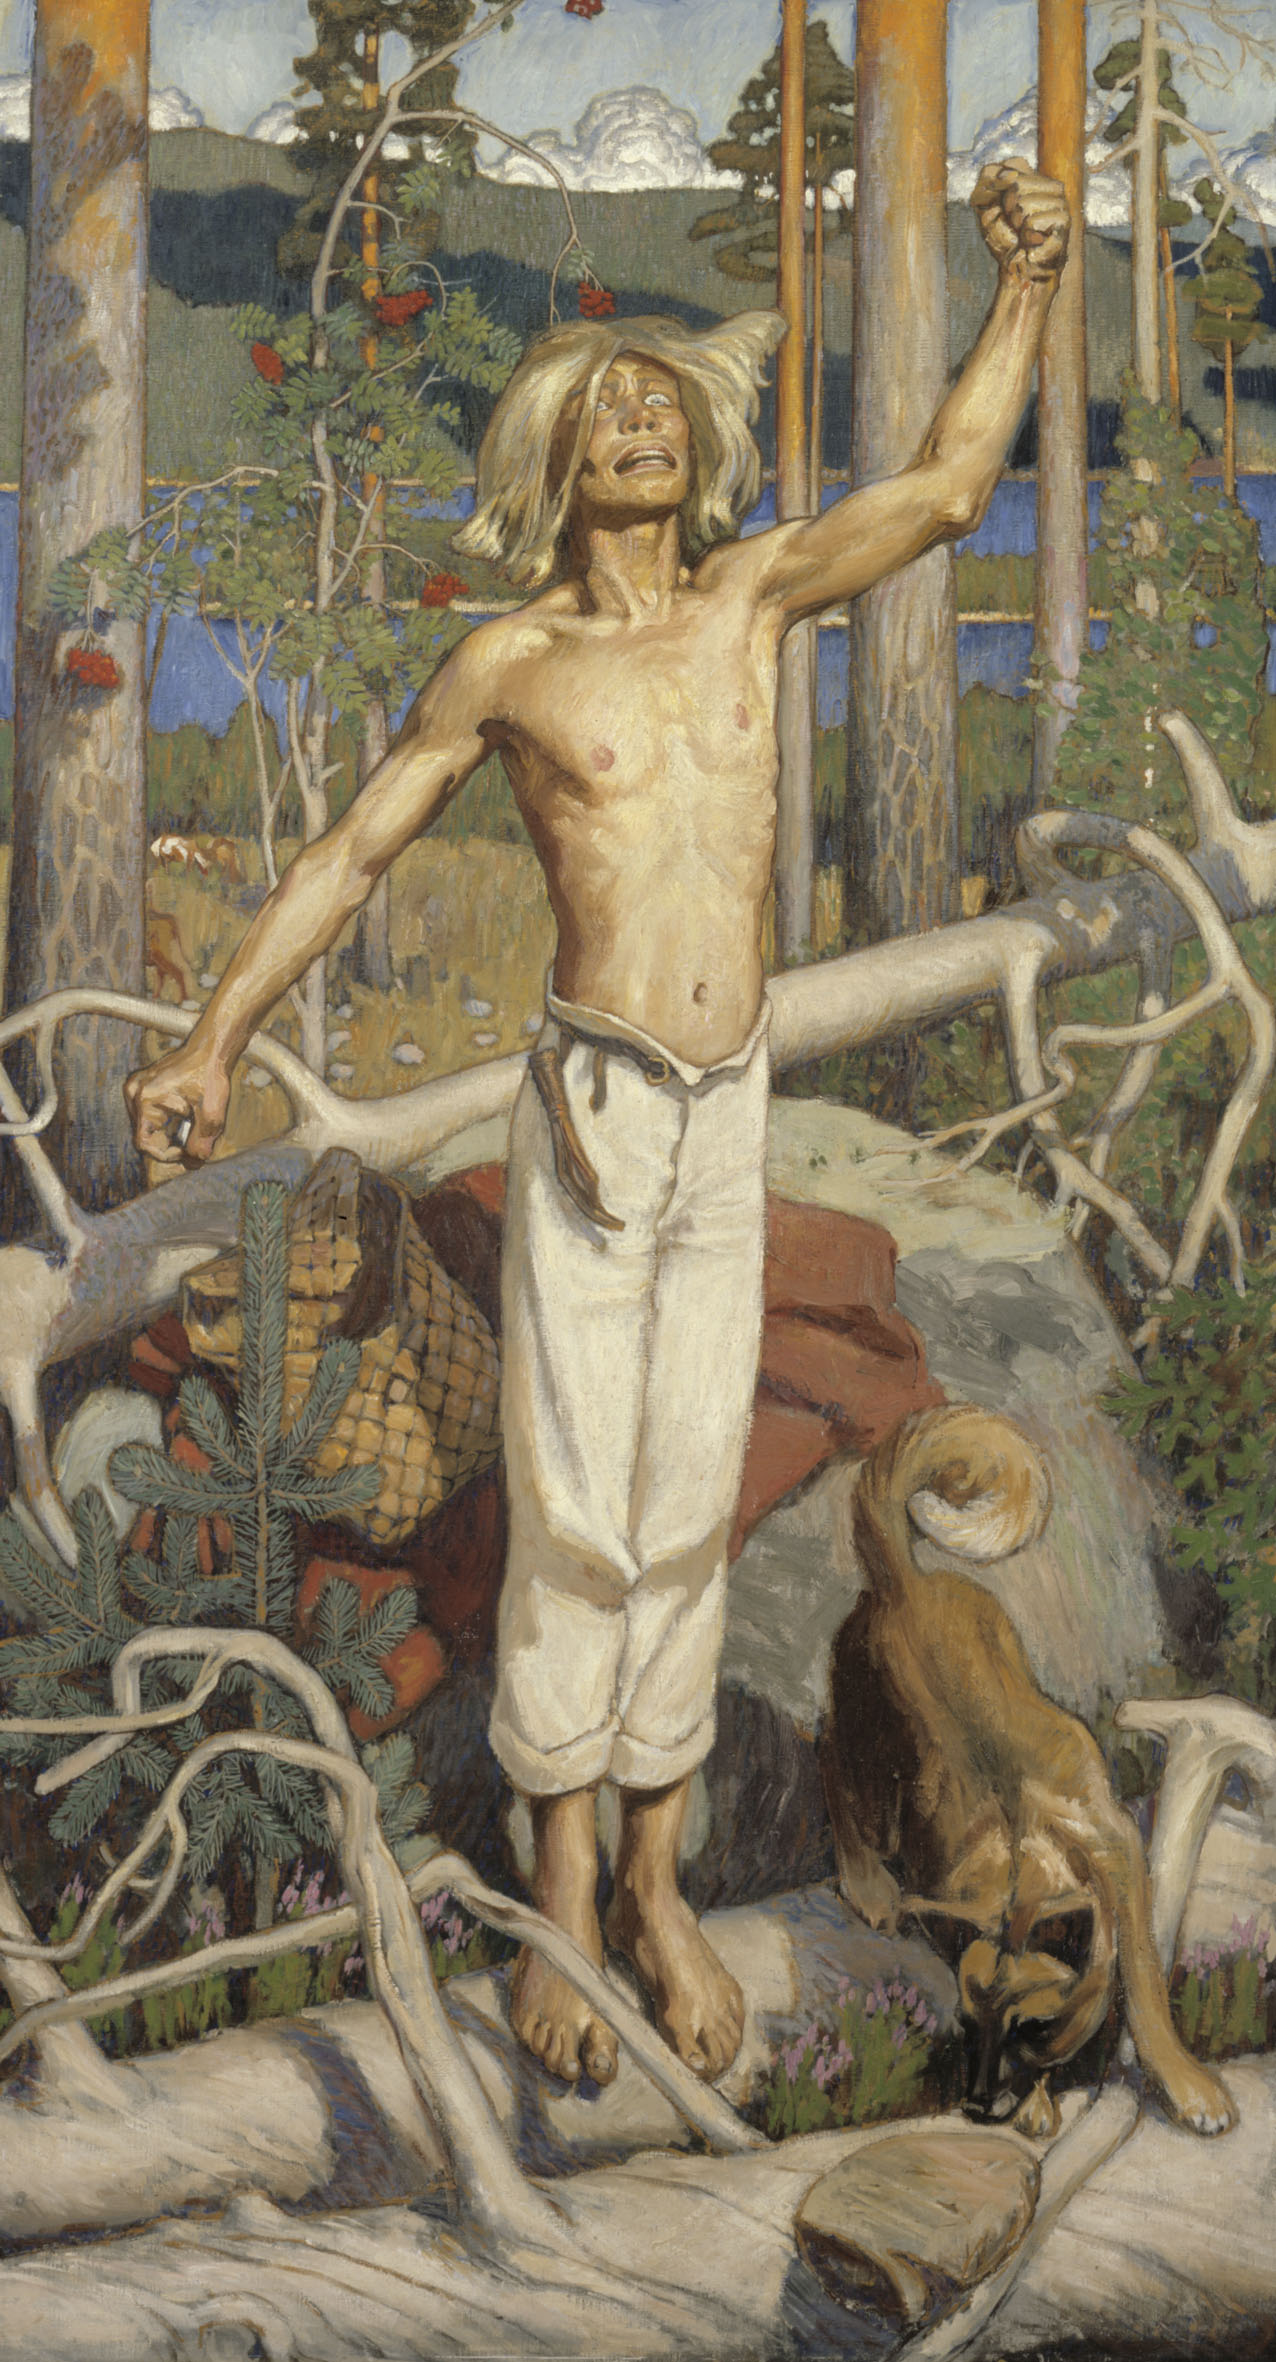
\includegraphics[width=1.00\textwidth]{./img/kullervo.png}
%		\caption{Kullervon kirous Akseli Gallen-Kallela}
%		\label{fig:kullervo}
	\end{figure}
	
	% Ensimmäinen runo

\chapter*{Ensimmäinen Runo}

\colorini{M}{ieleni minun tekevi}, aivoni ajattelevi          \\
lähteäni laulamahan, saa'ani sanelemahan,				          	\\	
sukuvirttä suoltamahan, lajivirttä laulamahan.              \\
Sanat suussani sulavat, puhe'et putoelevat,                 \\
kielelleni kerkiävät, hampahilleni hajoovat.                \\
                                                            \\
Veli kulta, veikkoseni, kaunis kasvinkumppalini!            \\
Lähe nyt kanssa laulamahan, saa kera sanelemahan            \\
yhtehen yhyttyämme, kahta'alta käytyämme!                   \\
Harvoin yhtehen yhymme, saamme toinen toisihimme            \\
näillä raukoilla rajoilla, poloisilla Pohjan mailla.        \\
                                                            \\
Lyökämme käsi kätehen, sormet sormien lomahan,              \\
lauloaksemme hyviä, parahia pannaksemme,                    \\
kuulla noien kultaisien, tietä mielitehtoisien,             \\
nuorisossa nousevassa, kansassa kasuavassa:                 \\
noita saamia sanoja, virsiä virittämiä                      \\
vyöltä vanhan Väinämöisen, alta ahjon Ilmarisen,            \\
päästä kalvan Kaukomielen, Joukahaisen jousen tiestä,       \\
Pohjan peltojen periltä, Kalevalan kankahilta.              \\
                                                            \\
Niit' ennen isoni lauloi kirvesvartta vuollessansa;         \\
niitä äitini opetti väätessänsä värttinätä,                 \\
minun lasna lattialla eessä polven pyöriessä,               \\
maitopartana pahaisna, piimäsuuna pikkaraisna.              \\
Sampo ei puuttunut sanoja eikä Louhi luottehia:             \\
vanheni sanoihin sampo, katoi Louhi luottehisin,            \\
virsihin Vipunen kuoli, Lemminkäinen leikkilöihin.          \\
                                                            \\
Viel' on muitaki sanoja, ongelmoita oppimia:                \\
tieohesta tempomia, kanervoista katkomia,                   \\
risukoista riipomia, vesoista vetelemiä,                    \\
päästä heinän hieromia, raitiolta ratkomia,                 \\
paimenessa käyessäni, lasna karjanlaitumilla,               \\
metisillä mättähillä, kultaisilla kunnahilla,               \\
mustan Muurikin jälessä, Kimmon kirjavan keralla.           \\
                                                            \\
Vilu mulle virttä virkkoi, sae saatteli runoja.             \\
Virttä toista tuulet toivat, meren aaltoset ajoivat.        \\
Linnut liitteli sanoja, puien latvat lausehia.              \\
                                                            \\
Ne minä kerälle käärin, sovittelin sommelolle.              \\
Kerän pistin kelkkahani, sommelon rekoseheni;               \\
ve'in kelkalla kotihin, rekosella riihen luoksi;            \\
panin aitan parven päähän vaskisehen vakkasehen.            \\
                                                            \\
Viikon on virteni vilussa, kauan kaihossa sijaisnut.        \\
Veänkö vilusta virret, lapan laulut pakkasesta,             \\
tuon tupahan vakkaseni, rasian rahin nenähän,               \\
alle kuulun kurkihirren, alle kaunihin katoksen,            \\
aukaisen sanaisen arkun, virsilippahan viritän,             \\
kerittelen pään kerältä, suorin solmun sommelolta?          \\
                                                            \\
Niin laulan hyvänki virren, kaunihinki kalkuttelen          \\
ruoalta rukihiselta, oluelta ohraiselta.                    \\
Kun ei tuotane olutta, tarittane taarivettä,                \\
laulan suulta laihemmalta, vetoselta vierettelen            \\
tämän iltamme iloksi, päivän kuulun kunniaksi,              \\
vaiko huomenen huviksi, uuen aamun alkeheksi.               \\
                                                            \\
Noin kuulin saneltavaksi, tiesin virttä tehtäväksi:         \\
yksin meillä yöt tulevat, yksin päivät valkeavat;           \\
yksin syntyi Väinämöinen, ilmestyi ikirunoja                \\
kapehesta kantajasta, Ilmattaresta emosta.                  \\
                                                            \\
Olipa impi, ilman tyttö, kave luonnotar korea.              \\
Piti viikoista pyhyyttä, iän kaiken impeyttä                \\
ilman pitkillä pihoilla, tasaisilla tanterilla.             \\
                                                            \\
Ikävystyi aikojansa, ouostui elämätänsä,                    \\
aina yksin ollessansa, impenä eläessänsä                    \\
ilman pitkillä pihoilla, avaroilla autioilla.               \\
                                                            \\
Jop' on astuiksen alemma, laskeusi lainehille,              \\
meren selvälle selälle, ulapalle aukealle.                  \\
Tuli suuri tuulen puuska, iästä vihainen ilma;              \\
meren kuohuille kohotti, lainehille laikahutti.             \\
                                                            \\
Tuuli neittä tuuitteli, aalto impeä ajeli                   \\
ympäri selän sinisen, lakkipäien lainehien:                 \\
tuuli tuuli kohtuiseksi, meri paksuksi panevi.              \\
                                                            \\
Kantoi kohtua kovoa, vatsantäyttä vaikeata                  \\
vuotta seitsemän satoa, yheksän yrön ikeä;                  \\
eikä synny syntyminen, luovu luomatoin sikiö.               \\
                                                            \\
Vieri impi veen emona. Uipi iät, uipi lännet,               \\
uipi luotehet, etelät, uipi kaikki ilman rannat             \\
tuskissa tulisen synnyn, vatsanvaivoissa kovissa;           \\
eikä synny syntyminen, luovu luomatoin sikiö.               \\
                                                            \\
Itkeä hyryttelevi; sanan virkkoi, noin nimesi:              \\
"Voi poloinen, päiviäni, lapsi kurja, kulkuani!             \\
Jo olen joutunut johonki: iäkseni ilman alle,               \\
tuulen tuuiteltavaksi, aaltojen ajeltavaksi                 \\
näillä väljillä vesillä, lake'illa lainehilla!              \\
                                                            \\
"Parempi olisi ollut ilman impenä eleä,                     \\
kuin on nyt tätä nykyä vierähellä veen emona:               \\
vilu tääll' on ollakseni, vaiva värjätelläkseni,            \\
aalloissa asuakseni, veessä vierielläkseni.                 \\
                                                            \\
"Oi Ukko, ylijumala, ilman kaiken kannattaja!               \\
Tule tänne tarvittaissa, käy tänne kutsuttaessa!            \\
Päästä piika pintehestä, vaimo vatsanvääntehestä!           \\
Käy pian, välehen jou'u, välehemmin tarvitahan!"            \\
                                                            \\
Kului aikoa vähäisen, pirahteli pikkaraisen.                \\
Tuli sotka, suora lintu; lenteä lekuttelevi                 \\
etsien pesän sijoa, asuinmaata arvaellen.                   \\
                                                            \\
Lenti iät, lenti lännet, lenti luotehet, etelät.            \\
Ei löyä tiloa tuota, paikkoa pahintakana,                   \\
kuhun laatisi pesänsä, ottaisi olosijansa.                  \\
                                                            \\
Liitelevi, laatelevi; arvelee, ajattelevi:                  \\
"Teenkö tuulehen tupani, aalloillen asuinsijani?            \\
Tuuli kaatavi tupasen, aalto vie asuinsijani."              \\
                                                            \\
Niin silloin ve'en emonen, veen emonen, ilman impi,         \\
nosti polvea merestä, lapaluuta lainehesta                  \\
sotkalle pesän sijaksi, asuinmaaksi armahaksi.              \\
                                                            \\
Tuo sotka, sorea lintu, liiteleikse, laateleikse.           \\
Keksi polven veen emosen sinerväisellä selällä;             \\
luuli heinämättähäksi, tuoreheksi turpeheksi.               \\
                                                            \\
Lentelevi, liitelevi, päähän polven laskeuvi.               \\
Siihen laativi pesänsä, muni kultaiset munansa:             \\
kuusi kultaista munoa, rautamunan seitsemännen.             \\
                                                            \\
Alkoi hautoa munia, päätä polven lämmitellä.                \\
Hautoi päivän, hautoi toisen, hautoi kohta kolmannenki.     \\
                                                            \\
Jopa tuosta veen emonen, veen emonen, ilman impi,           \\
tuntevi tulistuvaksi, hipiänsä hiiltyväksi;                 \\
luuli polvensa palavan, kaikki suonensa sulavan.            \\
                                                            \\
Vavahutti polveansa, järkytti jäseniänsä:                   \\
munat vierähti vetehen, meren aaltohon ajaikse;             \\
karskahti munat muruiksi, katkieli kappaleiksi.             \\
                                                            \\
Ei munat mutahan joua, siepalehet veen sekahan.             \\
Muuttuivat murut hyviksi, kappalehet kaunoisiksi:           \\
munasen alainen puoli alaiseksi maaemäksi,                  \\
munasen yläinen puoli yläiseksi taivahaksi;                 \\
yläpuoli ruskeaista päivöseksi paistamahan,                 \\
yläpuoli valkeaista, se kuuksi kumottamahan;                \\
mi munassa kirjavaista, ne tähiksi taivahalle,              \\
mi munassa mustukaista, nepä ilman pilvilöiksi.             \\
                                                            \\
Ajat eellehen menevät, vuoet tuota tuonnemmaksi             \\
uuen päivän paistaessa, uuen kuun kumottaessa.              \\
Aina uipi veen emonen, veen emonen, ilman impi,             \\
noilla vienoilla vesillä, utuisilla lainehilla,             \\
eessänsä vesi vetelä, takanansa taivas selvä.               \\
                                                            \\
Jo vuonna yheksäntenä, kymmenentenä kesänä                  \\
nosti päätänsä merestä, kohottavi kokkoansa.                \\
Alkoi luoa luomiansa, saautella saamiansa                   \\
selvällä meren selällä, ulapalla aukealla.                  \\
                                                            \\
Kussa kättä käännähytti, siihen niemet siivoeli;            \\
kussa pohjasi jalalla, kalahauat kaivaeli;                  \\
kussa ilman kuplistihe, siihen syöverit syventi.            \\
                                                            \\
Kylin maahan kääntelihe: siihen sai sileät rannat;          \\
jaloin maahan kääntelihe: siihen loi lohiapajat;            \\
pä'in päätyi maata vasten: siihen laitteli lahelmat.        \\
                                                            \\
Ui siitä ulomma maasta, seisattelihe selälle:               \\
luopi luotoja merehen, kasvatti salakaria                   \\
laivan laskemasijaksi, merimiesten pään menoksi.            \\
                                                            \\
Jo oli saaret siivottuna, luotu luotoset merehen,           \\
ilman pielet pistettynä, maat ja manteret sanottu,          \\
kirjattu kivihin kirjat, veetty viivat kallioihin.          \\
Viel' ei synny Väinämöinen, ilmau ikirunoja.                \\
                                                            \\
Vaka vanha Väinämöinen kulki äitinsä kohussa                \\
kolmekymmentä keseä, yhen verran talviaki,                  \\
noilla vienoilla vesillä, utuisilla lainehilla.             \\
                                                            \\
Arvelee, ajattelevi, miten olla, kuin eleä                  \\
pimeässä piilossansa, asunnossa ahtahassa,                  \\
kuss' ei konsa kuuta nähnyt eikä päiveä havainnut.          \\
                                                            \\
Sanovi sanalla tuolla, lausui tuolla lausehella:            \\
"Kuu, keritä, päivyt, päästä, otava, yhä opeta              \\
miestä ouoilta ovilta, veräjiltä vierahilta,                \\
näiltä pieniltä pesiltä, asunnoilta ahtahilta!              \\
Saata maalle matkamiestä, ilmoillen inehmon lasta,          \\
kuuta taivon katsomahan, päiveä ihoamahan,                  \\
otavaista oppimahan, tähtiä tähyämähän!"                    \\
                                                            \\
Kun ei kuu kerittänynnä eikä päivyt päästänynnä,            \\
ouosteli aikojansa, tuskastui elämätänsä:                   \\
liikahutti linnan portin sormella nimettömällä,             \\
lukon luisen luikahutti vasemmalla varpahalla;              \\
tuli kynsin kynnykseltä, polvin porstuan ovelta.            \\
                                                            \\
Siitä suistui suin merehen, käsin kääntyi lainehesen;       \\
jääpi mies meren varahan, uros aaltojen sekahan.            \\
                                                            \\
Virui siellä viisi vuotta, sekä viisi jotta kuusi,          \\
vuotta seitsemän, kaheksan. Seisottui selälle viimein,      \\
niemelle nimettömälle, manterelle puuttomalle.              \\
                                                            \\
Polvin maasta ponnistihe, käsivarsin käännältihe.           \\
Nousi kuuta katsomahan, päiveä ihoamahan,                   \\
otavaista oppimahan, tähtiä tähyämähän.                     \\
                                                            \\
Se oli synty Väinämöisen, rotu rohkean runojan              \\
kapehesta kantajasta, Ilmattaresta emosta.			        		\\
	% Toinen runo

\chapter*{Toinen Runo}

\colorini{N}{ousi siitä Väinämöinen} jalan kahen kankahalle				\\
saarehen selällisehen, manterehen puuttomahan.                  \\
                                                                \\
Viipyi siitä vuotta monta, aina eellehen eleli                  \\
saaressa sanattomassa, manteressa puuttomassa.                  \\
                                                                \\
Arvelee, ajattelevi, pitkin päätänsä pitävi:                    \\
kenpä maita kylvämähän, toukoja tihittämähän?                   \\
                                                                \\
Pellervoinen, pellon poika, Sampsa poika pikkarainen,           \\
sep' on maita kylvämähän, toukoja tihittämähän!                 \\
                                                                \\
Kylvi maita kyyhätteli, kylvi maita, kylvi soita,               \\
kylvi auhtoja ahoja, panettavi paasikoita.                      \\
                                                                \\
Mäet kylvi männiköiksi, kummut kylvi kuusikoiksi,               \\
kankahat kanervikoiksi, notkot nuoriksi vesoiksi.               \\
                                                                \\
Noromaille koivut kylvi, lepät maille leyhke'ille,              \\
tuomet kylvi tuorehille, raiat maille raikkahille,              \\
pihlajat pyhille maille, pajut maille paisuville,               \\
katajat karuille maille, tammet virran vieremille.              \\
                                                                \\
Läksi puut ylenemähän, vesat nuoret nousemahan.                 \\
Kasvoi kuuset kukkalatvat, lautui lakkapäät petäjät.            \\
Nousi koivupuut noroilla, lepät mailla leyhke'illä,             \\
tuomet mailla tuorehilla, katajat karuilla mailla,              \\
katajahan kaunis marja, tuomehen hyvä he'elmä.                  \\
                                                                \\
Vaka vanha Väinämöinen kävi tuota katsomahan                    \\
Sampsan siemenen aloa, Pellervoisen kylvämiä.                   \\
Näki puut ylenneheksi, vesat nuoret nousneheksi;                \\
yks' on tammi taimimatta, juurtumatta puu Jumalan.              \\
                                                                \\
Heitti herjan valloillensa, olevillen onnillensa;               \\
vuotti vielä yötä kolme, saman verran päiviäki.                 \\
                                                                \\
Kävi siitä katsomahan viikon päästä viimeistäki:                \\
ei ole tammi kasvanunna, juurtununna puu Jumalan.               \\
                                                                \\
Niin näkevi neljä neittä, viisi veen on morsianta.              \\
Ne oli nurmen niitännässä, kastekorren katkonnassa              \\
nenässä utuisen niemen, päässä saaren terhenisen;               \\
mink' on niitti, sen haravoi, kaikki karhille veteli.           \\
                                                                \\
Tulipa merestä Tursas, uros aalloista yleni.                    \\
Tunki heinäset tulehen, ilmivalkean väkehen;                    \\
ne kaikki poroksi poltti, kypeniksi kyyetteli.                  \\
                                                                \\
Tuli tuhkia läjänen, koko kuivia poroja.                        \\
Saip' on siihen lemmen lehti, lemmen lehti, tammen              \\
terho,                                                          \\
josta kasvoi kaunis taimi, yleni vihanta virpi;                 \\
nousi maasta mansikkaisna, kasvoi kaksihaarukkaisna.            \\
                                                                \\
Ojenteli oksiansa, levitteli lehviänsä.                         \\
Latva täytti taivahalle, lehvät ilmoille levisi:                \\
piätti pilvet juoksemasta, hattarat hasertamasta,               \\
päivän peitti paistamasta, kuuhuen kumottamasta.                \\
                                                                \\
Silloin vanha Väinämöinen arvelee, ajattelevi:                  \\
oisko tammen taittajata, puun sorean sortajata?                 \\
Ikävä inehmon olla, kamala kalojen uia                          \\
ilman päivän paistamatta, kuuhuen kumottamatta.                 \\
                                                                \\
Ei ole sitä urosta eikä miestä urheata,                         \\
joka taisi tammen kaata, satalatvan langettoa.                  \\
                                                                \\
Siitä vanha Väinämöinen itse tuon sanoiksi virkki:              \\
"Kave äiti, kantajani, luonnotar, ylentäjäni!                   \\
Laitapa ve'en väkeä  veessä on väkeä paljo                      \\
tämä tammi taittamahan, puu paha hävittämähän                   \\
eestä päivän paistavaisen, tieltä kuun kumottavaisen!"          \\
                                                                \\
Nousipa merestä miesi, uros aallosta yleni.                     \\
Ei tuo ollut suuren suuri eikä aivan pienen pieni:              \\
miehen peukalon pituinen, vaimon vaaksan korkeuinen.            \\
                                                                \\
Vaski- oli hattu hartioilla, vaskisaappahat jalassa,            \\
vaskikintahat käessä, vaskikirjat kintahissa,                   \\
vaskivyöhyt vyölle vyötty, vaskikirves vyön takana:             \\
varsi peukalon pituinen, terä kynnen korkeuinen.                \\
                                                                \\
Vaka vanha Väinämöinen arvelee, ajattelevi:                     \\
on miesi näkemiänsä, uros silmänluontiansa,                     \\
pystyn peukalon pituinen, härän kynnen korkunainen!             \\
                                                                \\
Siitä tuon sanoiksi virkki, itse lausui, noin nimesi:           \\
"Mi sinä olet miehiäsi, ku, kurja, urohiasi?                    \\
Vähän kuollutta parempi, katonutta kaunihimpi!"                 \\
                                                                \\
Sanoi pikku mies merestä, uros aallon vastaeli:                 \\
"Olen mie mokoma miesi, uros pieni, veen väkeä.                 \\
Tulin tammen taittamahan, puun murskan                          \\
murentamahan."                                                  \\
                                                                \\
Vaka vanha Väinämöinen itse tuon sanoiksi virkki:               \\
"Ei liene sinua luotu, eipä luotu eikä suotu                    \\
ison tammen taittajaksi, puun kamalan kaatajaksi."              \\
                                                                \\
Sai toki sanoneheksi; katsahtavi vielä kerran:                  \\
näki miehen muuttunehen, uuistunehen urohon!                    \\
Jalka maassa teutaroivi, päähyt pilviä pitävi;                  \\
parta on eessä polven päällä, hivus kannoilla takana;           \\
syltä oli silmien välitse, syltä housut lahkehesta,             \\
puoltatoista polven päästä, kahta kaation rajasta.              \\
                                                                \\
Hivelevi kirvestänsä, tahkaisi tasatereä                        \\
kuutehen kovasimehen, seitsemähän sieran päähän.                \\
                                                                \\
Astua lykyttelevi, käyä kulleroittelevi                         \\
lave'illa lahkehilla, leve'illä liehuimilla.                    \\
Astui kerran keikahutti hienoiselle hietikolle,                 \\
astui toisen torkahutti maalle maksankarvaiselle,               \\
kolmannenki koikahutti juurelle tulisen tammen.                 \\
                                                                \\
Iski puuta kirvehellä, tarpaisi tasaterällä.                    \\
Iski kerran, iski toisen, kohta kolmannen yritti;               \\
tuli tuiski kirvehestä, panu tammesta pakeni:                   \\
tahtoi tammi kallistua, lysmyä rutimoraita.                     \\
                                                                \\
Niin kerralla kolmannella jopa taisi tammen kaata,              \\
ruhtoa rutimoraian, satalatvan lasketella.                      \\
Tyven työnnytti itähän, latvan laski luotehesen,                \\
lehvät suurehen suvehen, oksat puolin pohjosehen.               \\
                                                                \\
Kenpä siitä oksan otti, se otti ikuisen onnen;                  \\
kenpä siitä latvan taittoi, se taittoi ikuisen taian;           \\
kenpä lehvän leikkaeli, se leikkoi ikuisen lemmen.              \\
Mi oli lastuja pirannut, pälähellyt pälkäreitä                  \\
selvälle meren selälle, lake'ille lainehille,                   \\
noita tuuli tuuitteli, meren läikkä läikytteli                  \\
venosina veen selällä, laivasina lainehilla.                    \\
                                                                \\
Kantoi tuuli Pohjolahan. Pohjan piika pikkarainen               \\
huntujahan huuhtelevi, virutteli vaattehia                      \\
rannalla vesikivellä pitkän niemyen nenässä.                    \\
                                                                \\
Näki lastun lainehilla; tuon kokosi konttihinsa,                \\
kantoi kontilla kotihin, pitkäkielellä piha'an,                 \\
tehä noian nuoliansa, ampujan asehiansa.                        \\
                                                                \\
Kun oli tammi taittununna, kaatununna puu katala,               \\
pääsi päivät paistamahan, pääsi kuut kumottamahan,              \\
pilvet pitkin juoksemahan, taivon kaaret kaartamahan            \\
nenähän utuisen niemen, päähän saaren terhenisen.               \\
                                                                \\
Siit' alkoi salot silota, metsät mielin kasvaella,              \\
lehtipuuhun, ruohomaahan, linnut puuhun laulamahan,             \\
rastahat iloitsemahan, käki päällä kukkumahan.                  \\
                                                                \\
Kasvoi maahan marjanvarret, kukat kultaiset keolle;             \\
ruohot kasvoi kaikenlaiset, monenmuotoiset sikesi.              \\
Ohra on yksin nousematta, touko kallis kasvamatta.              \\
                                                                \\
Siitä vanha Väinämöinen astuvi, ajattelevi                      \\
rannalla selän sinisen, ve'en vankan vieremillä.                \\
Löyti kuusia jyviä, seitsemiä siemeniä                          \\
rannalta merelliseltä, hienoiselta hietiköltä;                  \\
kätki nää'än nahkasehen, koipehen kesäoravan.                   \\
                                                                \\
Läksi maata kylvämähän, siementä sirottamahan                   \\
vierehen Kalevan kaivon, Osmon pellon penkerehen.               \\
                                                                \\
Tirskuipa tiainen puusta: "Eipä nouse Osmon ohra,               \\
ei kasva Kalevan kaura ilman maan alistamatta,                  \\
ilman kasken kaatamatta, tuon tulella polttamatta."             \\
                                                                \\
Vaka vanha Väinämöinen teetti kirvehen terävän.                 \\
Siitä kaatoi kasken suuren, mahottoman maan alisti.             \\
Kaikki sorti puut soreat; yhen jätti koivahaisen                \\
lintujen leposijaksi, käkösen kukuntapuuksi.                    \\
                                                                \\
Lenti kokko halki taivon, lintunen ylitse ilman.                \\
Tuli tuota katsomahan: "Miksipä on tuo jätetty                  \\
koivahainen kaatamatta, puu sorea sortamatta?"                  \\
                                                                \\
Sanoi vanha Väinämöinen: "Siksipä on tuo jätetty:               \\
lintujen lepeämiksi, kokon ilman istumiksi."                    \\
                                                                \\
Sanoi kokko, ilman lintu: "Hyvinpä sinäki laait:                \\
heitit koivun kasvamahan, puun sorean seisomahan                \\
linnuille lepeämiksi, itselleni istumiksi."                     \\
                                                                \\
Tulta iski ilman lintu, valahutti valkeaista.                   \\
Pohjaistuuli kasken poltti, koillinen kovin porotti:            \\
poltti kaikki puut poroksi, kypeniksi kyyetteli.                \\
                                                                \\
Siitä vanha Väinämöinen otti kuusia jyviä,                      \\
seitsemiä siemeniä yhen nää'än nahkasesta,                      \\
koivesta kesäoravan, kesäkärpän kämmenestä.                     \\
                                                                \\
Läksi maata kylvämähän, siementä sirottamahan.                  \\
Itse tuon sanoiksi virkki: "Minä kylvän kyyhättelen             \\
Luojan sormien lomitse, käen kautta kaikkivallan                \\
tälle maalle kasvavalle, ahollen ylenevälle.                    \\
                                                                \\
"Akka manteren-alainen, mannun eukko, maan emäntä!              \\
Pane nyt turve tunkemahan, maa väkevä vääntämähän!              \\
Eip' on maa väkeä puutu sinä ilmoisna ikänä,                    \\
kun lie armo antajista, lupa luonnon tyttäristä.                \\
                                                                \\
"Nouse, maa, makoamasta, Luojan nurmi, nukkumasta!              \\
Pane korret korttumahan sekä varret varttumahan!                \\
Tuhansin neniä nosta, saoin haaroja hajota                      \\
kynnöstäni, kylvöstäni, varsin vaivani näöstä!                  \\
                                                                \\
"Oi Ukko, ylijumala tahi taatto taivahinen,                     \\
vallan pilvissä pitäjä, hattarojen hallitsija!                  \\
Piä pilvissä keräjät, sekehissä neuvot selvät!                  \\
Iätä iästä pilvi, nosta lonka luotehesta,                       \\
toiset lännestä lähetä, etelästä ennättele!                     \\
Vihmo vettä taivosesta, mettä pilvistä pirota                   \\
orahille nouseville, touoille tohiseville!"                     \\
                                                                \\
Tuo Ukko, ylijumala, taatto taivon valtiainen,                  \\
piti pilvissä keräjät, sekehissä neuvot selvät.                 \\
Iätti iästä pilven, nosti longan luotehesta,                    \\
toisen lännestä lähetti, etelästä ennätteli;                    \\
syrjin yhtehen sysäsi, lomituksin loukahutti.                   \\
Vihmoi vettä taivosesta, mettä pilvistä pirotti                 \\
orahille kasvaville, touoille tohiseville.                      \\
Nousipa oras okinen, kannonkarvainen yleni                      \\
maasta pellon pehmeästä, Väinämöisen raatamasta.                \\
                                                                \\
Jopa tuosta toisna päänä, kahen, kolmen yön perästä,            \\
viikon päästä viimeistäki vaka vanha Väinämöinen                \\
kävi tuota katsomahan kyntöänsä, kylvöänsä,                     \\
varsin vaivansa näköä: kasvoi ohra mieltä myöten,               \\
tähkät kuuella taholla, korret kolmisolmuisena.                 \\
                                                                \\
Siinä vanha Väinämöinen katseleikse, käänteleikse.              \\
Niin tuli kevätkäkönen, näki koivun kasvavaksi:                 \\
"Miksipä on tuo jätetty koivahainen kaatamatta?"                \\
                                                                \\
Sanoi vanha Väinämöinen: "Siksipä on tuo jätetty                \\
koivahainen kasvamahan: sinulle kukuntapuuksi.                  \\
Siinä kukkuos, käkönen, helkyttele, hietarinta,                 \\
hoiloa, hopearinta, tinarinta, riukuttele!                      \\
Kuku illoin, kuku aamuin, kerran keskipäivälläki,               \\
ihanoiksi ilmojani, mieluisiksi metsiäni,                       \\
rahaisiksi rantojani, viljaisiksi vieriäni!"                    \\
	
\end{document}